\section{tkz 代码的基本元素}

要使用这个宏包，你需要一些 \LATEX 和 \TIKZ 的知识。

在本节中，我们来看用 \tkzname{\tkznameofpack} 创建图形所使用的 \code{rules} 和 \code{symbols}。

\subsection{对象与语言}

 基本对象是点。你可以在任何时候用定义点时所给的名称来引用它（之后也可以给它另一个名称）。

新的点通过宏获得。\tkzname{\tkznameofpack} 宏的名称以 \code{tkz} 开头。主要有四类，以以下开头：
|\tkzDef...| |\tkzDraw...| |\tkzMark...| 和 |\tkzLabel...|。
使用的点作为参数放在圆括号中传入，而创建的点放在花括号中给出。

图形的代码放在 \tkzimp{tikzpicture} 环境中。


与 \TIKZ 不同，宏不能以“;”结尾。因此我们失去了 \tkzimp{path} 这一重要概念。不过，你可以在 \tkzname{\tkznameofpack} 宏之间放置一些 \TIKZ 代码。


在第一类中，|\tkzDefPoint| 定义固定点；稍后会详细研究。这里我们来看宏 |\tkzDefTriangle|。

这个宏将第三个点与一对点关联，以定义某个三角形：|\tkzDefTriangle(A,B)|。得到的点引用为 |tkzPointResult|，你可以选择另一个引用，例如用 |\tkzGetPoint{C}|。

|\tkzDefTriangle[euclid](A,B) \tkzGetPoint{C}|

圆括号用于传递参数：在 |(A,B)| 中，$A$ 和 $B$ 是用于定义第三个点的点。在 |{C}| 中，花括号用于获取新点。

要从以下类型中选择一种三角形：
  |equilateral|,  |isosceles right|, |half|, |pythagoras|, |school|, |golden or sublime|, |euclid|, |gold|, |cheops|...
 和 |two angles|，你只需在方括号中给出选项，例如：
 
\begin{minipage}{0.5\textwidth}
  \begin{tikzpicture}[scale=.5]
  \tkzDefPoints{0/0/A,8/0/B}
  \foreach \tr in {golden, equilateral}
  {\tkzDefTriangle[\tr](A,B) \tkzGetPoint{C}
  \tkzDrawPoint(C)
  \tkzLabelPoint[right](C){\tr}
  \tkzDrawSegments(A,C C,B)}
  \tkzDrawPoints(A,B)
  \tkzDrawSegments(A,B)
   \tkzLabelPoints(A,B)
  \end{tikzpicture}
\end{minipage}
\begin{minipage}{0.5\textwidth}
  \begin{tkzexample}[code only,small]
    \begin{tikzpicture}[scale=.5]
    \tkzDefPoints{0/0/A,8/0/B}
   \foreach \tr in {golden, equilateral}
    {\tkzDefTriangle[\tr](A,B) \tkzGetPoint{C}
    \tkzDrawPoint(C)
    \tkzLabelPoint[right](C){\tr}
    \tkzDrawSegments(A,C C,B)}
    \tkzDrawPoints(A,B)
    \tkzDrawSegments(A,B)
    \tkzLabelPoints(A,B)
    \end{tikzpicture}
  \end{tkzexample}
\end{minipage}

\subsection{记号与约定}

我特意选择了法国几何约定以及一些个人约定来描述所表示的对象。\tkzname{\tkznameofpack} 定义和绘制的对象是平面中的点、直线和圆。它们是欧几里得几何的基本对象，我们由此构建图形。

根据 \tkzimp{Euclid} 的观点，这些图形仅说明我们心灵所产生的纯粹概念。
因此点没有维度，因而没有真实的存在。同样，直线没有宽度，因而在现实世界中没有存在。我们所考虑的对象只是理想数学对象的表示。\tkzname{\tkznameofpack} 遵循古希腊人的步骤，用直尺和圆规获得几何作图。

以下是使用的记号：

\begin{itemize}
\item 点用小圆点或两条直线的交点（两条直线、一条直线和一个圆，或两个圆）来表示。在第二种情况下，点用十字表示。

\begin{tkzexample}[latex=6cm, small]     
  \begin{tikzpicture}       
    \tkzDefPoints{0/0/A,4/2/B}       
    \tkzDrawPoints(A,B)       
    \tkzLabelPoints(A,B)     
  \end{tikzpicture}    
\end{tkzexample}

或者

\begin{tkzexample}[latex=6cm, small]     
  \begin{tikzpicture}       
    \tkzSetUpPoint[shape=cross, color=red]       
    \tkzDefPoints{0/0/A,4/2/B}       
    \tkzDrawPoints(A,B)       
    \tkzLabelPoints(A,B)     
    \end{tikzpicture}    
    \end{tkzexample}  

一旦一个点存在，我们就可以给它一个标签，即拉丁字母表中的一个大写字母（有一些例外），例如 $A$、$B$ 或 $C$。例如：
\begin{itemize}
\item $O$ 是圆的圆心、旋转中心等；
\item $M$ 是中点；
\item $H$ 是高的垂足；
\item $P'$ 是 $P$ 经过变换后的像。
\end{itemize}

请注意，代码中点的引用名称可能与文本中指定它的标签不同：我们可以定义一个点 A 并给它标签 $P$。样式也不同：点 A 标注为 $A$。

\begin{tkzexample}[latex=6cm, small]     
  \begin{tikzpicture}       
    \tkzDefPoint(0,0){A}       
    \tkzDrawPoints(A)       
    \tkzLabelPoint(A){$P$}     
  \end{tikzpicture}    
\end{tkzexample}

例外：某些点，例如三角形各边的中点，共享一个性质，因此它们的名称也共享一个共同的字母。我们用 $M_a$、$M_b$ 和 $M_c$ 或 $M_A$、$M_B$ 和 $M_C$ 来表示这些点。

在代码中，这些点称为 M\_A、M\_B 和 M\_C。

另一个例外涉及中间作图点，它们不标注。它们在代码中通常用小写字母表示。

\item 线段用其两个端点放在方括号中来表示：$[AB]$。

\item 在欧几里得几何中，一条直线由两个点定义：$A$ 和 $B$ 定义直线 $(AB)$。我们也可以用希腊字母为直线命名，如 $(\delta)$ 或 $(\Delta)$，或用小写字母如 $d$ 或 $d'$。

\item 射线（半直线）写作 $[AB)$。

\item 直线之间的关系：如果 $(AB)$ 和 $(CD)$ 垂直，我们写作 $(AB) \perp (CD)$；如果它们平行，我们写作 $(AB) \parallelslant (CD)$。

\item 三角形 $ABC$ 各边的长度为 $AB$、$AC$ 和 $BC$。数也用小写字母表示，因此我们写作 $AB=c$、$AC=b$ 和 $BC=a$。字母 $a$ 也用于表示角；$r$ 常用于表示半径，$d$ 表示直径或距离，$l$ 表示长度。

\item 多边形用其顶点表示：$ABC$ 是三角形，$EFGH$ 是四边形。

\item 角一般以度为单位度量（例如 $60^\circ$）；在等边三角形 $ABC$ 中，我们写作 $\widehat{ABC}=\widehat{B}=60^\circ$。

\item 弧用其端点表示：如果 $A$ 和 $B$ 是一个圆上的两个点，我们写作 $\widearc{AB}$。

\item 如果不会混淆，圆写作 $\mathcal{C}$；$\mathcal{C}$ $(O~;~A)$ 表示以 $O$ 为圆心、经过点 $A$ 的圆；$\mathcal{C}$ $(O~;~1)$ 表示以 $O$ 为圆心、半径为 1 cm 的圆。

\item 三角形特殊直线的名称：我使用角平分线、外角平分线、中垂线（通常称为垂直平分线）、高、中线和陪中线这些术语。

\item ($x_1$,$y_1$) 是点 $A_1$ 的坐标，($x_A$,$y_A$) 是点 $A$ 的坐标。
\end{itemize}

\subsection{\tkzname{Set, Calculate, Draw, Mark, Label}}
本节也可以称为 \texttt{计算与绘图的分离}。

当用 \LATEX 准备文档时，其源代码分为两部分：导言区和文档正文。
用这种方法，可以以最少的工作量对文档进行结构化、设置样式和排版。
我提出一种类似的方法，用 \tkzname{\tkznameofpack} 创建图形。

第一部分定义固定点，第二部分创建新点：\tkzname{Set and Calculate} 是两个主要部分。然后剩下要做的就是绘制（或填充）、标记和标注。\tkzname{\tkznameofpack} 对于最后这些操作中的某些可能不够用，但你随时可以使用 \TIKZ。

最后一点我认为很重要的意见：尽量避免在代码中使用坐标。坐标只应在开头与固定点一起出现；此后使用点的引用。大多数宏都有 \tkzname{nodes} 或 \tkzname{with nodes} 选项。

最好在开头定义不同对象的样式。
\endinput
